\documentclass{article}
\usepackage[GBK]{ctex}
\usepackage{booktabs} % 用于表格
\usepackage{longtable} % 用于长表格
\usepackage{geometry} % 控制页面边距
\usepackage{color}
\usepackage{type1cm} 
\usepackage{graphicx} % 图片
\usepackage{listings} % code
\geometry{a4paper, margin=1.1in}

\title{
HKU-MSc Computer Science
Admission Test Compilation
}
\author{Weicong HUANG, stalwarthuang@outlook.com}
\date{December 2024}

\begin{document}

% \setlength{\parindent}{0pt} % 禁用段落缩进


\maketitle

% 注释
\vspace{-3.5em} % 调整声明与标题之间的间距
\begin{center}
\textit{The following questions represent a selection from the entrance examination for the MSc in Computer Science at The University of Hong Kong. 
They have been sourced from online and are intended for personal study, research and communication purposes only!.}
\end{center}
\vspace{2em} 

\section{Programming}


\noindent\textbf{(25Fall)(20 marks)} In a course, there is a reward scheme. A token will be given to students when he/she submitted an assessment. A green card will be offered after collected 10 tokens. A yellow card will be offered after collected 6 green cards. A white card will be offered after collected 2 yellow cards. You are required to write a program to read the number of tokens obtained. Then report the number of corresponding green card, yellow card and white card. Besides, the number of tokens that are required for obtaining a gold medal should be reported.

\noindent Sample Test case 1:
\begin{table}[h!]
\centering
\begin{tabular}{|p{3cm}|p{9.2cm}|}
\hline
\textbf{Input} & \textbf{Expected output} \\
\hline
\textbf{18} & 
\begin{tabular}{@{}c@{}}
You got 0 white card, 0 yellow card and 1 green card. \\
You need 222 tokens to get a gold medal.
\end{tabular} \\
\hline
\end{tabular}
\label{tab:example}
\end{table}

\noindent Sample Test case 2:
\begin{table}[h!]
\centering
\begin{tabular}{|p{3cm}|p{9.2cm}|}
\hline
\textbf{Input} & \textbf{Expected output} \\
\hline
\textbf{220} & 
\begin{tabular}{@{}c@{}}
You got 1 white card, 3 yellow cards and 22 green cards. \\
You need 20 tokens to get a gold medal.
\end{tabular} \\
\hline
\end{tabular}
\label{tab:example}
\end{table}

\noindent Sample Test case 3:
\begin{table}[h!]
\centering
\begin{tabular}{|p{3cm}|p{9.2cm}|}
\hline
\textbf{Input} & \textbf{Expected output} \\
\hline
\textbf{240} & 
\begin{tabular}{@{}c@{}}
Congratulations! You got a gold medal!
\end{tabular} \\
\hline
\end{tabular}
\label{tab:example}
\end{table}

\vspace{2\baselineskip}

\noindent\textbf{(25Fall)(20 marks)} Write a program that prints an equilateral triangle pattern with alternating digits (0s and ls). Your program should prompt the user to enter the size of the triangle (an integer $n$). The triangle should have $n$ lines. Each line should start with a digit that alternates between 0 and 1. The digits within each line should alternate between 0 and 1. The triangle should be equilateral, meaning each line is centered based on the longest line. \\ 

\noindent Sample Test case 1(red represents user input):
\begin{table}[h!]
\centering
\begin{tabular}{|p{3cm}|p{6cm}|}
\hline
\textbf{Input} & \textbf{Expected output} \\
\hline
\textbf{Size: \textcolor{red}{3}} & 
\begin{tabular}{@{}c@{}}
0 \\ 
1 0 \\ 
0 1 0 \\
\end{tabular} \\
\hline
\end{tabular}
\label{tab:example}
\end{table}
    

\vspace{2\baselineskip}

\noindent\textbf{(20 marks)} A positive integer \(n > 2\) is sacred if \(n = a^2 + b^3\) for some integers \(a\) and \(b\). Write a program (using either the programming language C, C++, Java, Python) that repeatedly asks the user to input a positive integer \(n\), and prints "YES" if it is sacred, and "NO" otherwise. The program stops if a negative integer is input.

\vspace{2\baselineskip} % 空两行

\noindent\textbf{(10 marks)} There are 150 cards, each with a different number written on it.The cards are arranged in a 15 x 10 grid such that each row is arranged in increasing order from left to right, and each column is arranged in increasing order from top to bottom. All cards are face down, making it impossible to see the numbers on them. Your task is to find a specific number $x$. You need to design a method that will allow you to find the card with number $x$ while turning up as few cards as possible. Additionally, if the number $x$ is not among the 150 cards, your method should be able to determine this. Describe your method in whatever way you feel comfortable (it is okay to use pseudocode or flowchart). What is the minimum number of cards your method will need to turn up in the worst-case scenario? Justify your answer.

\vspace{2\baselineskip}

\noindent Suppose $is\_prime(m)$ is a build-in function that returns "True" if $m$ is a prime number, and returns "False" otherwise.
A positive integer is special if it has two factors $f$ and $f+2$ where both $f$ and $f$ are prime. Write a complete program (in any programming language) that inputs an positive integer $x$, and prints "Yes" if x is special, and "No" otherwise. You may use the function  in your program. (Note: 1 is a factor any any positive integer.)

\vspace{5\baselineskip}


\noindent The following method for finding the square-root of a positive number is known to the ancient Babylonians (1500 BC).

\hangindent=2em % 设置悬挂缩进
\hangafter=1     % 从第二行开始生效
\textit{1.Make an initial guess. Guess any positive number $x_0$.}\\
\textit{2.Improve the guess: Apply the formula $x_1 = (x_0+S/x_0) / 2$. The number $x_1$ is a better estimate to the square root of $S$.}\\
\textit{3.Iterate until convergence: Apply the formula $x_(n+1) = (x_n+S/x_n) / 2$ until the process converges (i.e., the difference between $x_(n+1)-x_n$is smaller than some small numbers.}

\noindent a.(8\%) Apply the above method to find the square-root of $S=20$. Your answer needs to show all the values of $x_0, x_1, ...$\\
\noindent b.(12\%) Write a program (either in C, C++, Java or Python)that implements the above algorithm to find square of a positive, i.e., it asks the user to inputs a positive number $S$, and then prints the square root of $S$.

\vspace{2\baselineskip}

\noindent A bag contains $n$ balls, and the number of balls that can be removed at a time is limited to 1, 2, or 3. Provide a list of all possible scenarios that could result from this process.

\vspace{2\baselineskip}

\noindent A series $a_1, a_2, a_3...a_n$, if satisfied $a_1 < a_2 <a_3 <...< a_i > a_(i+1) > ... > a_n$, is said to be a single-peaked series, if the series is single-peaked, then print "Yes", otherwise "No".

\vspace{2\baselineskip}

\noindent Write a program in any of the following programming languages: C, C++, Python, Java. The program should take a decimal integer as input and display its binary representation. For example, if the input is $12$, then the program should print $1100$.

\vspace{2\baselineskip}

\noindent Given a string, output the sum of the numbers in the string.\\
\textit{\fontsize{9pt}{12pt}\selectfont e.g. $12iloveHKU3student4 -> 12+3+4$}

\vspace{2\baselineskip}

\noindent \textbf{(30marks)} In discrete mathematics, Ramsey's theorem states that for any positive integer $k$, there is an integer $m$ such that in any party with at least $m$ guests, one of the following statements must be true:

\hangindent=2em % 设置悬挂缩进
\hangafter=1     % 从第二行开始生效
\textit{(1)There are at least $k$ guests who know each other.}\\
\textit{(2)There are at least $k$ guests who do not know each other.}

For example, for $k=3$, then in any party of at least 6 guests, either there are 3 guests who know each other, or there are 3 guests who do not know each other. This question asks you to write a program (using either Python,C,C++, Java) to help verify Ramsey's theorem. The input of the program is organized as follows:


\indent $\cdot$ The first line of the input has an integer $m$, followed by $m$ lines of string, each representing a guest (so there are totally $m$ guests for this input).\\
\indent $\cdot$ Then, there is another line of integer $n$, followed by $n$ lines of pair of guests (guest $a$ and guest $b$ know each other if and only if there is a line of pair $a, b$ in the input).\\
\indent $\cdot$ Then, there is a line containing an integer $k$.
For the output, your program should print a set of $k$ guests who knows each other, and if there is no such set, the program should print a set of $k$ guests who do not know each other.\\

\vspace{2\baselineskip}

\noindent Write a program (using either Python, Java, C or C++) that (i) inputs a positive integer n, (ii) prints a line of consecutive integers from 2 to n (inclusively), and then (iii) repeatedly inputs a prime number f and do the following until $f = 2$:

prints a line of integers constructed by removing from the previously printed line those integers that have an odd number of factor $f$. (For example, the integer $24 = 2 \times 2 \times 2 \times 3$ has an odd number of factor 2.)

Following is an example on the execution of the program:
\begin{lstlisting}
20 
2 3 4 5 6 7 8 9 10 11 12 13 14 15 16 17 18 19 20 
3 
2 4 5 7 8 9 10 11 13 14 16 17 18 19 20 
2 
4 5 7 9 11 13 16 17 19 20 
\end{lstlisting}

\vspace{1\baselineskip}





\section{Mathematics \& Discrete mathematics}

\noindent \textbf{(25Fall)(10 marks)} Which of the following statements are true? \\
\indent (a) $\{a\}$ \\ 
\indent (b) ${3 \in \{3\}}$ \\
\indent (c) ${4 \in \{1, 2, 3, \{4\}\} }$ \\
\indent (d) ${\emptyset \in \{\emptyset\}}$ \\
\indent (a) ${\emptyset \in {\{\{\emptyset\}\}}}$ \\



\vspace{2\baselineskip}

\noindent \textbf{(25Fall)(10 marks)} Which of the following are propositions? \\
\indent (a) A cow has four legs.\\
\indent (b) Do not stand on the flowers.\\
\indent (c) There is no greatest prime number.\\
\indent (d) 7 > 47.\\
\indent (e) As white as a sheet.\\
\indent (f) It will rain somewhere in Shanghai on Nov 16, 2025.\\
\indent (g) Is that a reasonable argument?\\
\indent (h) If 2+2=5 then the sky is green.\\

\vspace{3\baselineskip}

\noindent \textbf{(25Fall)(10 marks)} Prove the following statement by Mathematical Induction for all positive integers $n$.
$$ \sum_{k=1}^{n}(2 k-1)=n^{2} $$

\vspace{3\baselineskip}


\noindent \textbf{(25Fall)(10 marks)} \\
(a) Find the second derivative of $y$ with respect to $x$. \indent $y = 6cosx + 7sinx$ \\
(b) Compute \indent  $\int x^{2} \cos x d x$.

\vspace{3\baselineskip}

\noindent \textbf{(25Fall)(10 marks)} \\
(a) Find the second derivative of $y$ with respect to $x$. \indent $y = 4x + \sqrt{(1-x)}$ \\
(b) Compute \indent  $\int x^{2} \cos x d x$.

\vspace{3\baselineskip}

\noindent \textbf{(10 marks)} The figure shows the shaded region bounded by the curve $y=x^3+x^2-6x$ and the $x-axis$ for $-2 \le x \le 3$.\\
\indent (a)Find the -intercepts of the curve.\\
\indent (b)Find the area of the shaded region.\\ 

\hfill
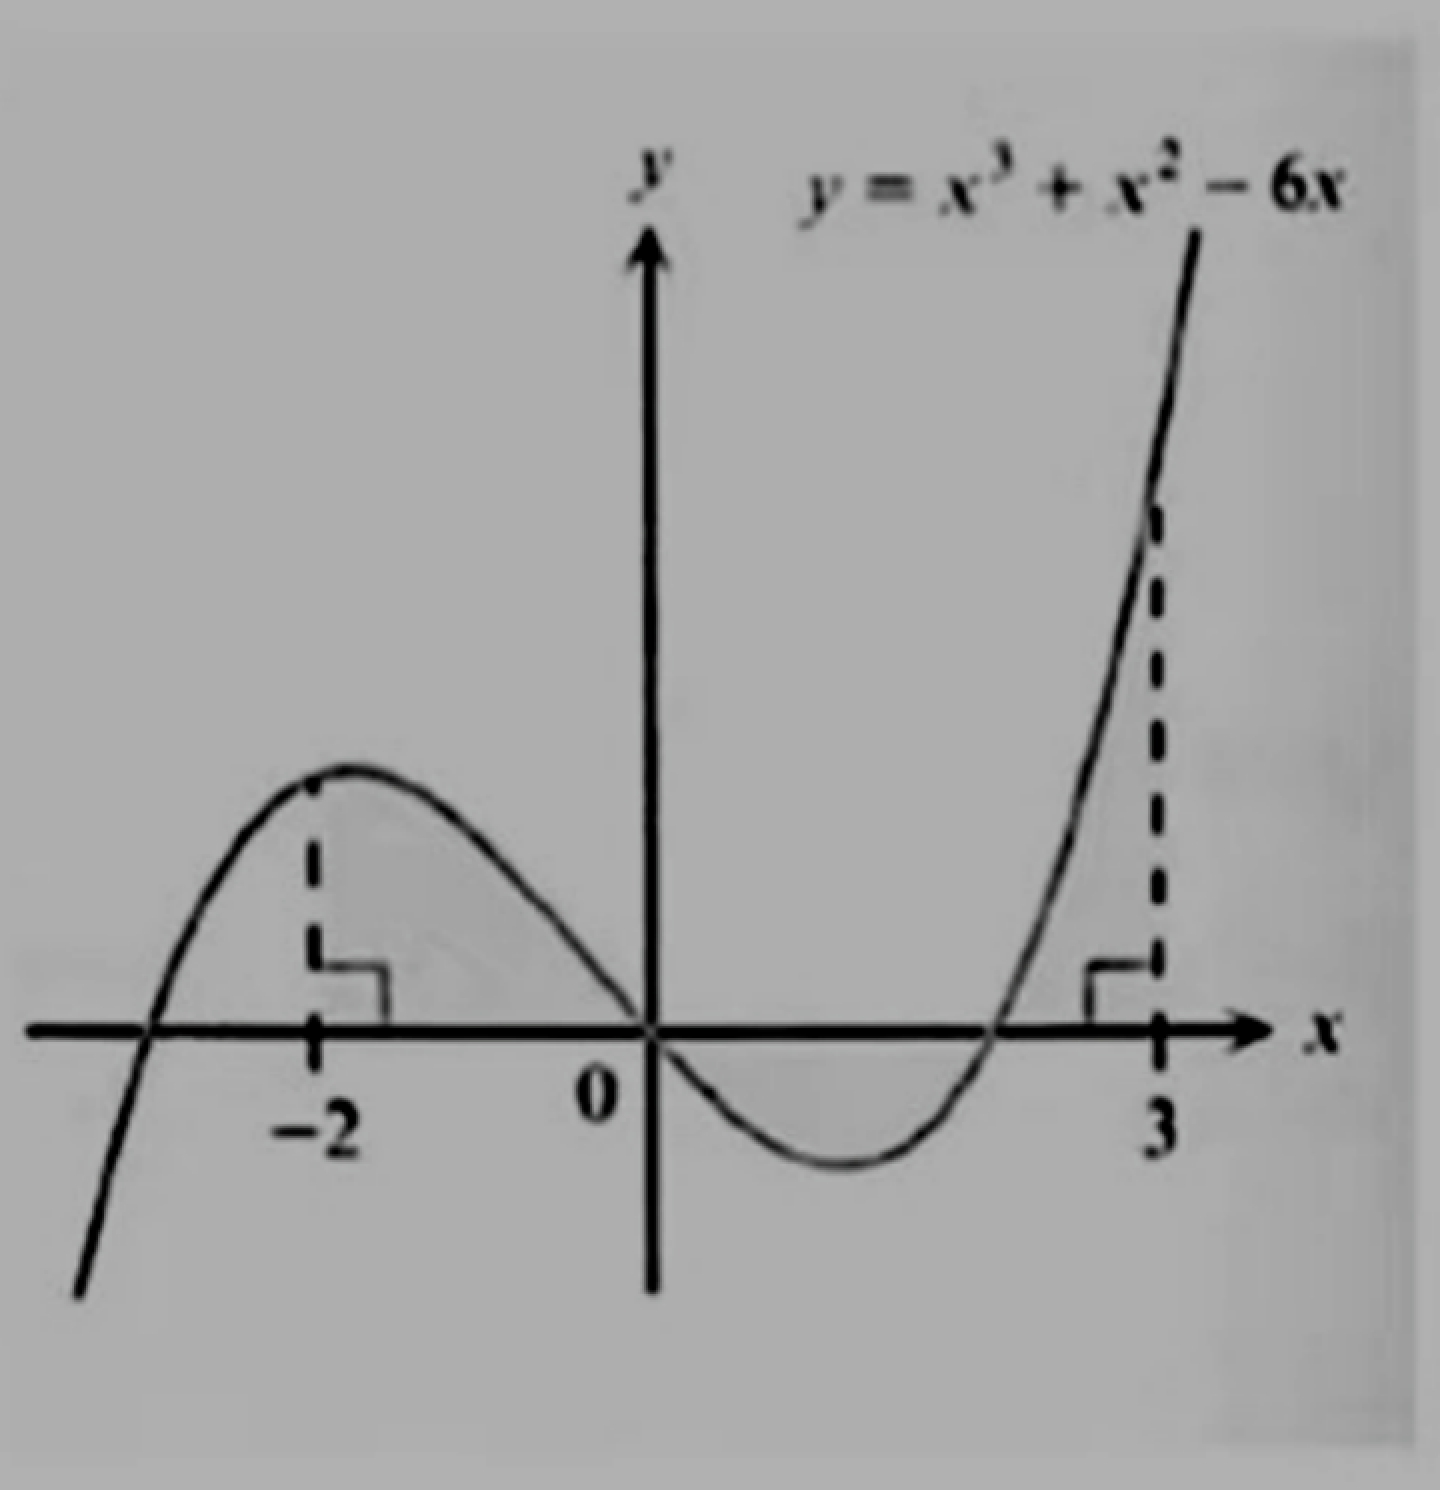
\includegraphics[width=5cm, height=3cm]{graph1.jpg}

\vspace{3\baselineskip}

\noindent \textbf{(10 marks)} Find the second derivative for each of the following functions with respect to $x$.\\
\indent (a) $y=\sqrt{2x+1}$\\
\indent (b) $e^{x^2}$

\vspace{3\baselineskip}

\noindent \textbf{(10 marks)} Compute \indent $$\frac{\mathrm{d} \frac{(1-x)^3}{2-3x} }{\mathrm{d} x} \indent \indent \int_{0}^{\sqrt{x}}(t+1)^\frac{1}{2} dt $$

\vspace{3\baselineskip}

\noindent \textbf{(10 marks)} Compute 
$$ \frac{\mathrm{d} (x-\sqrt{2x + 1} )^3}{\mathrm{d} x} \mid _{x=4} $$ \\
$$ \int xe^x dx $$ \\
$$ ({\frac{5z-4}{z+4} })' $$ \\
$$ \int \frac{2x+1}{\sqrt[]{x^2 + x + 7}}dx $$ \\
$$ \int \frac{7}{{(2x+1)(x-3)}}dx $$ 

\vspace{3\baselineskip}

\noindent Given a dataset: $\{x_1, x_2, x_3,...,x_n\}$.\\
(a) write down the formula for the standard deviation(标准差).\\
(b) let $p$ be the standard deviation of this dataset. Now, if each item is decreased by dividing a constant $c$, i.e. the dataset becomes $\{\frac{x_1}{c}, \frac{x_2}{c}, \frac{x_3}{c},...,\frac{x_n}{c}\}$, what is the new standard deviation? Or explain why it cannot be determined.

\vspace{3\baselineskip}

\noindent \textbf{(10\%)} Using calculus, find the area of the region bounded by $x = 3y^2+y$, the $y-axis$ and the lines $x=0$ and $y = 4$, as shown in the figure.\\

\hfill
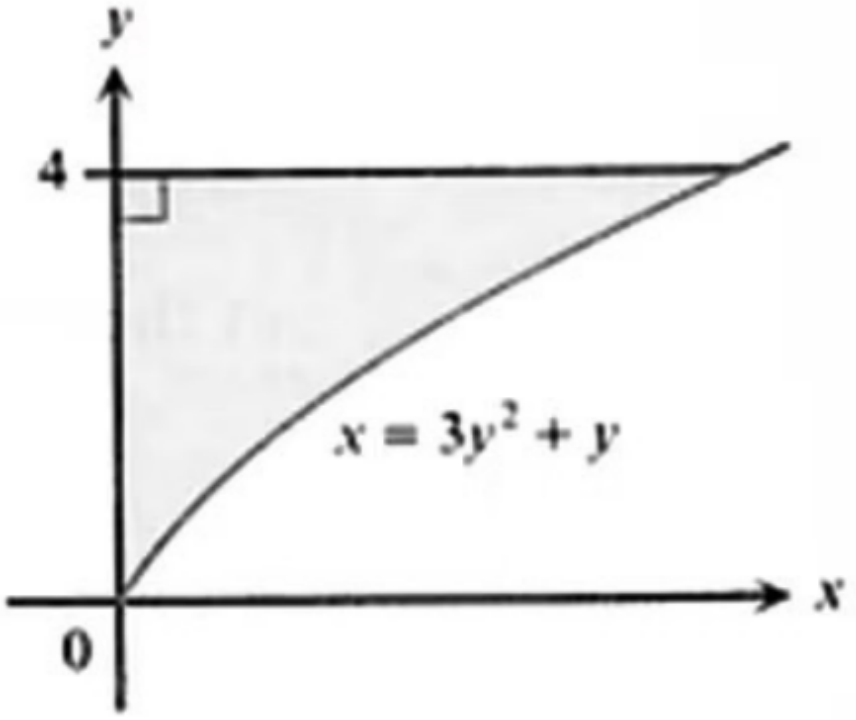
\includegraphics[width=5cm, height=3cm]{graph2.png}

\vspace{3\baselineskip}

\noindent Prove by Mathematical Induction that for every positive integer $n$.
$$1\times2+2\times3+3\times4+...+n\times(n+1) = \frac{n(n+1)(n+2)}{3}$$

\vspace{6\baselineskip}


\section{Probability Theory}

\noindent \textbf{(25Fall)(10 marks)} Two events A and B with the probabilities $P(A)=0.5$, $P(B)=0.3$ and $P(A \cup B) = 0.1$. Calculate:\\
(a) $P(A | B)$ \\
(b) $P(A | A \cup B)$ \\
(c) $P(A \cap B | A \cup B)$ \\

\vspace{3\baselineskip}

\noindent \textbf{(25Fall)(10 marks)} Two fair dice are tossed and $X$ equals the larger of the two scores obtained. Find the probability function of $X$ and determine $E(X)$. \\

\vspace{3\baselineskip}

\noindent \textbf{(10 marks)} The probability that "a vehicle crossing the Grand Tunnel is a private car" is 0.35. Suppose there are 6 vehicles crossing the tunnel. Let $X$ be the random variable representing the number of private cars among the 6 vehicles.\\
\indent (a) Find Pr($X = 4$) \\
\indent (b) Find Pr($X \ge 4$) \\
\indent (c) Find Pr($X \le 3$) \\

\vspace{3\baselineskip}

\noindent Assume that the probability a child is a boy is 0.6 and that the sexes of children born into a family are independent. What is the probability that a family of five children has \\
\indent 1. exactly three boys? \\
\indent 2. at least one girl? \\
\indent 3. all children of the same sex? \\

\vspace{3\baselineskip}

\noindent What is the probability that two people chosen at random were born on the same day of the week(e.g., both on Monday).\\

\vspace{3\baselineskip}

\noindent \textbf{(10 marks)} On a flight of HKA airline, 5\% of the passengers take the first-classseats. Among those passengers, 30\% of them are Hong Kong citizens. It is known that 60\% of the first-class passengers who are Hong Kong citizens have become members of HKA  airline, and the airline only accept Hong Kong citizens as their members.If a passenger is  randomly chosen from the passenger list of the flight, find the probability that the passenger takes a first-class seat but is not a member of HKA airline.\\

\vspace{3\baselineskip}

\noindent There is a blood test for the new H3M1 disease. If a person having the disease is tested, the test has a probability 8\% of showing a negative result. If a person not having the disease tested, the test has a probability 4\% of showing a positive result. It is estimated that 3\% of the people in the city have the H3MI disease. Find the probability that a person actually has the disease if he gets a positive result in the blood test.

\vspace{3\baselineskip}

\noindent The probability of a hacker attacking a company's computer and the computer being poisoned is 1\%. There is a testing organization that can test for computer viruses. If the computer is infected with a virus, the test result will be positive; if the computer is not infected with a virus, the test result will be negative. Now, if a computer detection result is positive, what is the probability that the computer has a virus?

\vspace{3\baselineskip}

\noindent Recall that the variance of a sequence of numbers is used to measure the variability of the numbers. We can extend the definition to measure the variability of two sequences numbers $x_1, x_2,...,x_n$ and $y_1, y_2,...,y_n$ by defining the covariance of these two sequences as follows:
$$\frac{(x_1-\bar{x})(y_1-\bar{y}) + (x_2-\bar{x})(y_2-\bar{y}) + ... + (x_n-\bar{x})(y_n-\bar{y})}{n}$$
where $\bar{x} = \frac{x_1 + x_2 + x_3 + ... + x_n}{n}$ and $\bar{y} = \frac{y_1 + y_2 + y_3 + ... + y_n}{n}$ are the average of the $x_i's$ and the $y_i's$ respectively. Intuitively, if the covariance of the two sequences is (significantly) greater than zero, they are positively related, i.e., the greater values of one variable mainly corresponding with the greater values of the other values, and if the covariance is (significantly) smaller than zero, they are negatively related. If their covariance is zero, the two sequences do not have relation.\\
This question asks you to show that the above intuition is not always true by completing the following two sequences $X = [-3, -2, -1, 0, 1, 2, ?]$ and $Y = [3, 2, 1, 0, ?, ?, ?]$ such that (a) the two sequences are closely related, i.e., given a value of $x$, we can determine the corresponding value of $y$ correctly, and (b) the covariance of the two sequences is zero. Justify your answer.


\section{IQ}

\noindent There are 12 stacks of 12 coins, and there is exactly one stack in which all its coins are fake (i.e., counterfeit), and all the coins in the remaining 11 stacks are genuine (not fake). Every genuine coin weighs 10 grams, and every fake coin weighs 11 grams. You have a  scale that can tell you the total weight of any selection of coins. Design a method that uses  the scale to find the stack of fake coins. (An obvious solution uses the scale 12 times. Look  for one that uses the scale fewer than 12 times.)

\end{document}